\documentclass{article}
\usepackage[utf8]{inputenc}
\usepackage{graphicx}
\usepackage{caption}
\usepackage{subcaption}
\usepackage{listings}
\usepackage{xcolor}
\usepackage{placeins}
\usepackage{fancyhdr}

\newcommand\enunciat[2][blue]{\textcolor{#1}{\emph{#2}}}
\newcommand\subject{Tipologia i cicle de vida de les dades}
\newcommand\activity{PRAC1}

\title{\large \subject \\ \activity}
\author{Josep Alòs Pascual, Daniel Galan Vilella}
\date{\today}
\makeatletter

\pagestyle{fancy}
\lhead{\subject}
\rhead{\activity}
\rfoot{Josep Alòs Pascual\\Daniel Galan Vilella}

\begin{document}
\maketitle

\section{Descripció del projecte}
\subsection{Context i inspiració}
\enunciat{Explicar en quin context s'ha recol·lectat la informació. Explicar per
què el lloc web triat proporciona aquesta informació. Explicar per què és
interessant aquest conjunt de dades i quines preguntes es pretenen respondre.}

Ens trobem en els inicis de la nostra vida laboral, on el nostre poder
adquisitiu és superior que en la nostra època d'estudiants de grau. Cansats de
freqüentar els mateixos bars i restaurants autoanomenats 'low cost', ens hem
començat a interessar en restaurants d'un altre tipus.

Utilitzant la pàgina de TripAdvisor hem anat explorant nous restaurants. Tot i
això, com a bons informàtics, no som amics de les tasques manuals repetititves.
Aprofitant aquesta pràctica, hem decidit que podem solucionar aquest problema
mitjançant les tècniques d'analisi de dades, que estem aprenent en aquest
master, de forma que ens pugui recomanar restaurants nous sense haver de pensar
nosaltres on anar.

TripAdvisor és l'opció ideal per obtenir dades sobre restaurants ja que té
informació sobre (1) la ubicació, (2) el preu aproximat, (3) comentaris i
puntuacions, (4) i detalls de la seva cuina.


\subsection{Descripció del dataset}
\enunciat{Definir un títol pel dataset. Triar un títol que sigui descriptiu.}

Restaurants Lleida

\enunciat{Descripció del dataset. Desenvolupar una descripció breu del conjunt
de dades que s'ha extret (és necessari que aquesta descripció tingui sentit amb
el títol triat).}

Aquest dataset conté dades relatives als restaurants de Lleida. Aquesta
informació fa referència a dos blocs: (1) dades informatives del restaurant
(horaris, ubicació, telèfon\dots), i (2) dades de qualitat (puntuacions i
comentaris). En l'apartat~\ref{sec:contingut} es mostra en detall quines dades
es guarden.

Aquestes dades s'han extret de TripAdvisor, i per tant no són dades
proporcionades pel restaurant directament sinó que estan basades en les
aportacions dels clients, fet que pot aportar soroll però a la vegada
informació més imparcial.


\subsection{Representació gràfica}
\enunciat{Presentar una imatge o esquema que identifiqui el dataset visualment}
En la figura~\ref{fig:plot} podem veure la distribució de les puntuacions
dels diferents restaurants del dataset.

\begin{figure}[h]
	\centering
	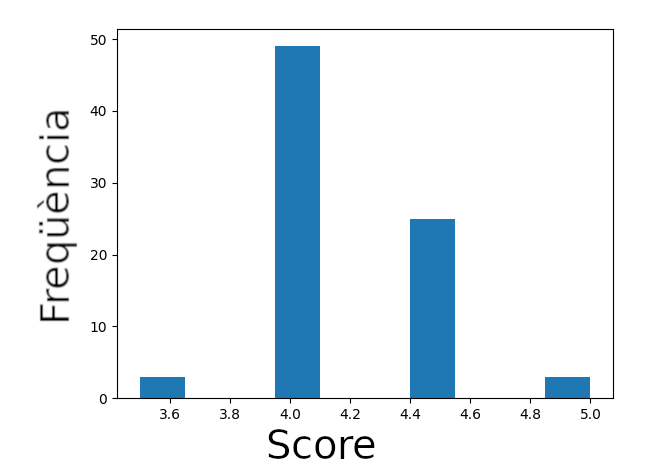
\includegraphics{plot.png}
	\caption{Distribució de les puntuacions dels restaurants}
	\label{fig:plot}
\end{figure}

\subsection{Contingut}\label{sec:contingut}
\enunciat{Explicar els camps que inclou el dataset, el període de temps de les
dades i com s'ha recollit.}

El dataset estarà separat en dos fitxers. En el primer s'inclourà la informació
referent als restaurants, i el segon sobre els comentaris dels usuaris. S'ha
decidit separar els dos conjunts per tal de mantenir la consistència dins d'un
mateix fitxer i evitar tenir dades duplicades.

\paragraph{Dataset 1: restaurants}
Aquest dataset conté informació sobre els restaurants. Les dades i el seu tipus
es mostren en la taula~\ref{table:dataset1_data}.

\begin{table}[h]
	\centering
	% TODO review hipenation
    \begin{tabular}{|p{.2\textwidth}|p{.1\textwidth}|p{.6\textwidth}|}
		\hline
        Nom       & Tipus  & Descripció \\\hline\hline
        Nom       & string & Nom del restaurant. \\\hline
        Adreça    & string & Direcció del restaurant. \\\hline
        Telèfon   & string & Telèfon del restaurant. \\\hline
        Puntuació & float  & La puntuació que té el restaurant. Aquesta
                             puntuació és la mitjana de les puntuacions de
                             menjar, servei, preu, i atmosfera. El seu valor
                             va d'1 a 5, i pot ser un nombre decimal. \\\hline
        Puntuació menjar & float & \\\hline
        Puntuació servei & float & \\\hline
        Puntuació preu & float & \\\hline
        Puntuació atmòsfera & float & \\\hline
		Rang de preu & string & El rang de preus que es troben els plats.\\\hline
        Detalls cuina & string & Detalls de la cuina d'aquest restaurant (estil,
                                 plats\dots). \\\hline
        Certificat excelència & boolean & Si el restaurant té un certificat
                                          d'excelència. \\\hline
    \end{tabular}
    \caption{Dades de restaurants}
    \label{table:dataset1_data}
\end{table}

\paragraph{Dataset 2: comentaris} % TODO
Aquest dataset contindrà la informació sobre els comentaris d'un restaurant.
Les dades guardades i el seu tipus es mostren en la
taula~\ref{table:dataset1_data}.

\begin{table}[h]
	\centering
    \begin{tabular}{|p{.2\textwidth}|p{.1\textwidth}|p{.7\textwidth}|}
		\hline
        Nom            & Tipus  & Descripció \\\hline\hline
        Restaurant     & string & Identificador del restaurant\\\hline
        Usuari         & string & L'usuari que ha escrit el comentari \\\hline
        Titol          & string & El titol del comentari \\\hline
        Text           & string & El contingut del comentari \\\hline
        Data de visita & date   & La data de la visita (mes i any) \\\hline
        Puntuació      & int    & La puntuació que ha donat aquest usuari
								  \\\hline
        Resposta       & string & Resposta del restaurant (pot existir o no)
								  \\\hline
    \end{tabular}
    \caption{Dades dels comentaris}
    \label{table:dataset2_data}
\end{table}

Aquestes dades s'han col·leccionat al novembre de 2019. S'han agafat dades de
comentaris de l'últim any per reduïr la quantitat d'informació amb la que es
treballava, però el codi proporciona un paràmetre per generar datasets més
amb altres dates.

Referent als restaurants, TripAdvisor proporciona dades en una llista ordenada
per rellevància. Per tant, s'ha limitat als 80 primers restaurants d'aquesta
llista, pel mateix motiu esmentat anteriorment. Aquest valor també es
parametritzable.
\linebreak

Per tal de recollir aquestes dades, s'ha fet un \textit{web scrapping} de la
pàgina de la llista de restaurants de Lleida, i per cada restaurant s'ha agafat
l'enllaç de la seva pàgina de detalls i se n'ha analitzat el contingut. Per
últim, aquestes dades s'han guardat en dos fitxers \textit{csv}.

\subsection{Agraïments}
\enunciat{Presentar el propietari del conjunt de dades. És necessari incloure
cites de recerca o anàlisis anteriors (si n'hi ha).}

El propietari d'aquestes dades és TripAdvisor, Inc.

\subsection{Llicència}
\enunciat{Seleccionar una d'aquestes llicències pel dataset resultant i explicar
el motiu de la seva selecció:
\begin{itemize}
    \item Released Under CC0: Public Domain License
    \item Released Under CC BY-NC-SA 4.0 License
    \item Released Under CC BY-SA 4.0 License
    \item Database released under Open Database License, individual contents
    under Database Contents License
    \item Other (specified above)
    \item Unknown License
\end{itemize}}

Aquestes dades són propietat de TripAdvisor, Inc. Segons la seva pàgina web,
qualsevol ús d'aquestes dades s'ha de consultar amb els seus creadors:
\begin{quote}
	Please note that any use of TripAdvisor content, with the exception of the
	self-service widgets, must be approved by TripAdvisor. For more information
	on the use of our self-service widgets, please see our Widget Terms of Use
	for specific requirements. For complete instructions about how to find and
	use self-service widgets, please refer to our Insights guide.
\end{quote}

Tot i això, sota la clàusula de \textit{Fair Use} del Copyright, entenem que
aquestes dades es poden fer servir de forma educativa durant un procès
d'aprenentatge. Per qualsevol altre ús de les dades s'ha de contactar amb els
seus propietaris. Per tant, aquest dataset està protegit sota una llicència de
Copyright, propietat de TripAdvisor, Inc.


\section{Taula de contribucions}
Les contribucions a aquest projecte es poden veure a la
taula~\ref{table:contribucions}.
\begin{table}[h]
	\centering
    \begin{tabular}{|l|l|}
		\hline
        Contribucions & Signa \\\hline\hline
        Recerca prèvia & DGV, JAP \\\hline
        Redacció de les respostes & DGV, JAP \\\hline
        Desenvolupament del codi & DGV, JAP \\\hline
    \end{tabular}
    \caption{Taula de contribucions}
    \label{table:contribucions}
\end{table}
\end{document}
